\documentclass[sigconf]{acmart}

\usepackage{hyperref}

\usepackage{endfloat}
\renewcommand{\efloatseparator}{\mbox{}} % no new page between figures

\usepackage{booktabs} % For formal tables

\settopmatter{printacmref=false} % Removes citation information below abstract
\renewcommand\footnotetextcopyrightpermission[1]{} % removes footnote with conference information in first column
\pagestyle{plain} % removes running headers


\begin{document}
\title{Big Data and Artificial Neural Networks}



\author{Bharat Mallala}
\affiliation{%
  \institution{Indiana University}
  \city{Bloomington, IN 47408} 
  \country{USA}}
\email{bmallala@iu.edu}


% The default list of authors is too long for headers}
\renewcommand{\shortauthors}{B. Trovato et al.}


\begin{abstract}
Big data is often referred as a problem of dealing with large data sets. With the advancements in computational science and the recent evolution of Artificial Intelligence(AI) and Machine Learning, huge volumes of data are being generated every day. Simultaneously the computational resources needed to process and analyze this data is trying to catch up with the rapidly growing data and for the most part have succeeded. In today's world, there is a large dependency on Neural networks for dealing with problems in AI and Data analysis. Big data and its applications can be used to address various issues that arise with Artificial Neural Networks(ANN). 
\end{abstract}

\keywords{I523, hid215, Artificial Neural Networks, Machine Learning, Artificial Intelligence, Data Analysis, Perceptron, Back propagation, Feed forward.}


\maketitle

\section{Introduction}

Artificial Neural Networks are often referred as a Multi-layer Neural Network where each node in the network is a Perceptron. It often mics the human brain, i.e. it works in a similar fashion. Advancements in ANN's and its ability to solve complex problems at a relatively faster rate than the traditional approaches have made it the top choice for solving the usually NP-hard AI problems. "Visual analysis systems will all require a neural network behind them, and that involves a lot of computing power"\cite{Anderson2017} quoted Anderson. This explains the efficiency of Neural networks in solving problems and analysis. ANN's take a series of inputs from the users and map them accordingly to find reasonable patterns in data.

Certainly, with these advancements comes huge volumes of data which needs to be stored and processed efficiently. This is where Big data comes into picture with its ability to store and process large data sets of any kind, for example, audio, video, images, text etc in relatively less time. "s Big Data Analytics is an effective and capable way to, not only work with these data but understand its meaning, providing inputs for assertive analysis and predictive actions."\cite{Barros2016} quotes Victor P Barros in his paper.

Artificial Neural Networks usually consists of three primary layers, an input layer, output layer, hidden layer. There may be multiple layers of perceptrons within the hidden layer. From the figure 1 we can see the three layers of the ANN. The input layer takes in the input as a set of features and its corresponding weights and the output layer returns a predicted value. All the calculations are done in the hidden layer. The ANN's typically use the feedforward algorithm combined with back propagation for its calculation. The figure below shows the structure of ANN with the three layers. The network initially feeds forward to the very end and generates an output from the initial set of features and weights. It then back propagates using Gradient descent and recalculates the wights for each iteration. The algorithm finally stops of the difference in weights from one iteration to the other is not greater than a predefined threshold. We then test this on the training set and evaluate the performance of the network.


\section{ANN's with Big data in Pharmacology}

\subsection{Pharmacology}
ANN's with its advancements over the years has been one of the most effective ways in prediction and extracting useful features in the field of Pharmacology. "Pharmacology is the branch of medicine concerned with the uses, effects, and modes of action of drugs"\cite{www-wiki}. In this study the data sets comprise of three parts, training data set, testing data set, and validation data set. The ANN's are used to differentiate between active compounds and inactive ones which help in the selection of compounds for use in life-saving drugs.\cite{LucasAntonPastur-Romay2016}

\subsection{History}
A lot of research has been conducted in the field of Pharmacology from the late 1980's. Researchers have acknowledged the power of ANN's and have started using it for prediction and classification of robust compounds and materials.\cite{LucasAntonPastur-Romay2016} But till the early 2000's the use of ANN's have slowed down due to the lack of enough data for training and testing the networks. But with the advancements in big data from the early 2000's the use of ANN's for predictive analytics have raised from the ashes.Big data provided a means of effectively storing huge volumes of the Pharmacological and bioinformatics data and to effectively process them. The effectiveness of big data lies in its ability to store and process the structured, semi-structured and unstructured data. Figure 2 shows the various stages of big data.



\subsection{Method and Analysis}
A series of processes are carried from the initial state till we get the final predicted outcome. It all starts with the selection of desired features based on the type of analysis to be carried out. This step is called Feature extraction. Hadoop(HDFS) with the ability to store large volumes of data is used to store the large data sets pertaining to Pharmacology. It is a distributed file system with a single name node and various data nodes. Feature extraction process is applied to data on HDFS and the apt features are extracted. The next phase is the initialization of weights, where we need to initialize the weights for the first iteration of the backpropagation algorithm. This is done using an unsupervised pre-training process.

Once the features of interest are extracted and we have the initial weights, then the ANN's are trained over these feature sets to extract patterns from data and gain insights from them. In general ANN's are classified into a number of modules, for example, Deep Neural Networks(DNN), Convolution Neural Networks(CNN), Deep Recurrent Neural Networks(DRNN)\cite{LucasAntonPastur-Romay2016}. 


DRNN is the most prominent when it comes to dealing with Pharmacology data. Generally, a ANN does not have loops in its architecture i.e. the output of each layer acts as input to the next layer in a chain-like manner. But in a DRNN there are loops within the network. i.e. the output of a layer will act as an input to the previous layer forming a loop, hence the name Recurrent. In Pharmacology DRNN's are used to predict the molecular properties or robust compounds. Figure 3 below shows the architecture of a DRNN.


\subsection{Role of Big data}

Due the vastness of the data sets the traditional algorithms needs to be modified to run the analysis more efficiently. The best approach to deal with this is parallel processing. Spark a component of big data has a set of Machine learning libraries through which the parallel processing is carried on multiple nodes of the network. Spark has an advantage over the other Big data components such as PIG, Hive, Map reduce with ease of writing code as well as user adoption towards it. The data here gets distributed across various data nodes in the cluster where the name node has the metadata pertaining to the data in the data nodes. So the ML algorithms are applied to the data from all the data node where the processing part is carried across multiple machines in a parallel manner. This helps in faster processing and lesser load on the machines. The below figure shows the big data architecture. \cite{www-google}


\section{ANN's for Pattern Recognition in Cloud gaming using Big Data}

\subsection{Cloud based games}
With the enhanced usage of smartphone and gaming consoles, cloud-based gaming is getting more and more prominent among many users from the past decade. All the traffic from such Cloud-based games and handles over the internet. With more intensive games being created, a large volume of different varieties of data is been generated and this data should be effectively handled for a smooth and pleasant user experience. In any Cloud-based game, there are mainly two players, the client and the server. The client sends requests to the server and the server replies with the relevant information. Some of the cloud-based gaming platforms are Gaikai and OnLive in the early 2000's, while today the most widely used ones are Sony's PlayStation and Microsoft's XBox.

\subsection{Role of Big data}
Since all these games are being played in real time, a lot of data is being generated every minute across all the major gaming platforms. This data comprises of audio, video, text which need to be stored, processed and analyzed in real time. This is stored information is helpful both for the company which made the game for further improvement of the game and the player's community for discussing tactics and comparing results.
Figure 4 shows the Architecture and various components of big data.

Game Telemetry is the statistical data associated with Cloud-based games which most of the companies collect in a timely manner and conduct some rigorous analysis on. This is data is usually in large volumes which cannot be addressed by traditional methods. This where Big data comes into the picture with its ability to store and process such data. This is data also helps is finding patterns in data using some pattern recognition algorithm with ANN which is usually run on robust platforms, and gaining insights from the same. These are generally associated with the Hadoop atmosphere along with the integration of ANN's, where the Cloud-based gaming is carried out in parallel across multiple nodes\cite{Barros2016}.

\subsection{Artificial Neural networks for Analysis}

With the power and efficiency of ANN's in predictive analysis there most prominently used in Cloud-based gaming platforms. The dataset used for this study was taken from World of Warcraft game where each player is associated with an avatar which they play with. The ANN's are used analyze user behavior based on their avatar names in the games and classify them as low, medium and high. In this case, the ANN's are used for classification into the three classes stated. The approach involves analysis patterns on how players select their avatars and time they play with them along with the skills and attributes of each of the avatars using Big data tools. The networks used for this approach is the Multi-layer Feedforward network along with Backpropagation.The networks consist of 4 input neurons, 7 hidden neurons, and 1 output neuron. The output neuron is the class variable. The weights, in this case, are initialized at random and the Backpropagation algorithm recalculated the weights in each iteration. This ANN classified the class variable with an accuracy of 84 percent. 


\section{Conclusions}

Artificial Neural Network is one of the most prominent Machine learning tool used both for classification and regression. Various modulations of ANN's are used based on the type of analysis to be carried out and the class variable. Some of them are Deep Neural Networks(DNN), Convolution Neural Networks(CNN), Deep Recurrent Neural Networks(DRNN). ANN's with its ability to solve complex problems needs a good amount of training data to train the model. Big data and its application and components provided the means to store and process large volumes of the various type of data. A lot of analysis has been conducted in various fields of study with the integration of Big data with ANN's, some of which have been covered in this paper. Results from these studies have proves that the networks can be trained to recognize various patterns in data and learn from the new as it becomes available.







\begin{acks}

I would like to thank Dr. Gregor von Laszewski and the AI's for all the help they have provided for this paper.
\end{acks}



\bibliographystyle{ACM-Reference-Format}
\bibliography{report} 

\begin{figure}[htp]
    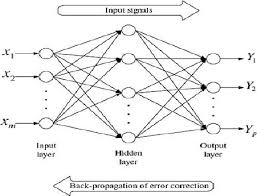
\includegraphics[width=0.8\textwidth]{images.jpg}
    \caption{Neural Network Architecture \cite{google}}
    \label{fig:figure1}
\end{figure}

\begin{figure}[htp]
    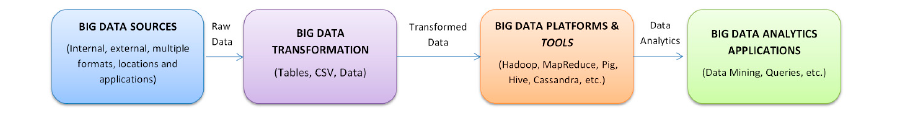
\includegraphics[width=0.8\textwidth]{images1.jpg}
    \caption{Stages of big data}
    \label{fig:figure2}
\end{figure}

\begin{figure}[htp]
    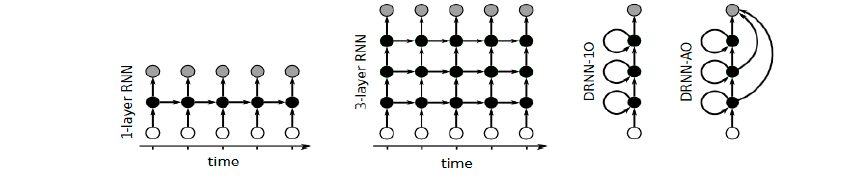
\includegraphics[width=0.8\textwidth]{images2.jpg}
    \caption{Architecture of DRNN}
    \label{fig:figure3}
\end{figure}

\begin{figure}[htp]
    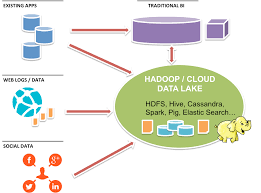
\includegraphics[width=0.8\textwidth]{images3.jpg}
    \caption{Big data Architecture and Components \cite{www-google}}
    \label{fig:figure4}
\end{figure}

\end{document}
